% [6~r\textsuperscript{o}] atque ibi versus cordis mucronem deflexa sinum dextrum a %sinistro in posteriore cordis superficie distinguebat.\pend
\pstart%
Dexter sinus multo \edtext{[brevior]}{\lemma{brevius}\Bfootnote{\textit{L \"{a}ndert Hrsg.}}}
erat quam sinister etiam proportione magis quam in vitulis ejusque caro mollior: paries exterior fere triplo minor: intus reperi sanguinem rubicundum, in sinistro vero nigrum et adustum, vena arteriosa aliquanto etiam mollior videbatur quam aorta, sed quod mirum, ejus cum aorta conjunctio tam plane evanuerat ut nulla ejus vestigia apparerent nisi tantum exigua ruga in vena arteriosa. Ipsa autem materia ex qua intermedius canalis factus fuerat in durum adipem videbatur esse conversa. Meatus vero ex cava in arteriam venosam plane erat etiam clausus; sed foramen adhuc instar fossae cujusdam ex parte cavae cernebatur, et rugae multae in medio transversim protuberantes; supra vero et infra excavatae ex parte arteriae venosae.
\pend%
% \vspace{1.0em}%
\pstart%
% \noindent%
Jam notavi os cordis satis durum, et quo secto
\edtext{medium rubebat,}{\lemma{}\Bfootnote{medium \textbar\ medium \textit{gestr.}\ \textbar\ rubebat, \textit{L}}}
tanquam ex medulla spongioso osse conclusa, erat autem
\edtext{hic}{\lemma{}\Afootnote{\textit{\"{U}ber} hic: hoc \Denarius \vspace{-4mm}}}
os vel potius haec duo ossa in radicibus aortae et plus quam mediam ejus orificii partem cingebant, unum quidem magis ab anteriore parte cordis inter orificium cavae et aortae habebat exordium et ibi cava arteriae proxima est quendam processum deorsum mittebat, pergebatque postea usque ad medium intervalli inter aortam et venam arteriosam, ibique nescio an alteri ossi jungeretur, vel potius ipsam cartilaginem factum ulterius progrediebatur ad usque finem illius interstitii, quod est inter aortam et venam
\edtext{arteriosam. Valvula}{\lemma{arteriosam}\Bfootnote{\textit{(1)}\ , ibique nescio an alteri ossi jungeretur, vel potius \textit{(2)}\ . Valvula \textit{L}}} 
autem ibi in isto intervallo pro vena arteriosa existens plane cartilaginea erat et fibrae longe duriores quam in sinistro ventriculo, adeo ut longe major inter cordis sinus appareret diversitas quam in vitulis.
\pend 
\pstart Non accurate distinctae erant valvulae arteriae venosae et licet duae caeteris majores apparerent in angulis; tamen etiam aliae duae esse videbantur, adeo ut 4 possent numerari.
\pend%
\pstart%
Caeterum pericardium adhaerebat ipsi cordi non tantum in basi sed etiam in parte posteriori a basi ad mucronem usque ad latitudinem 3 aut 4 digitorum; innumeris fibris
\pend
\newpage
\pstart\noindent ei erat consutum quae fibrae in extremitatibus duriores erant quam in medio atque in sinistra parte quam in dextra. In medio autem cordis inter istas fibras erat instar cujusdam glandulae pisi romani magnitudine et figura prominens album tuberculum, quod ibi intra ipsam cordis tunicam erat adnatum. Circumquaque vero pericardium erat adiposa quadam veluti spuma conspersum et contectum.
\pend%
\vspace{1.0em}% PR: Bitte diesen leeren Zeilenabstand behalten !!!
\pstart%
% \noindent% 
%\begin{wrapfigure}{l}{0.5\textwidth}
%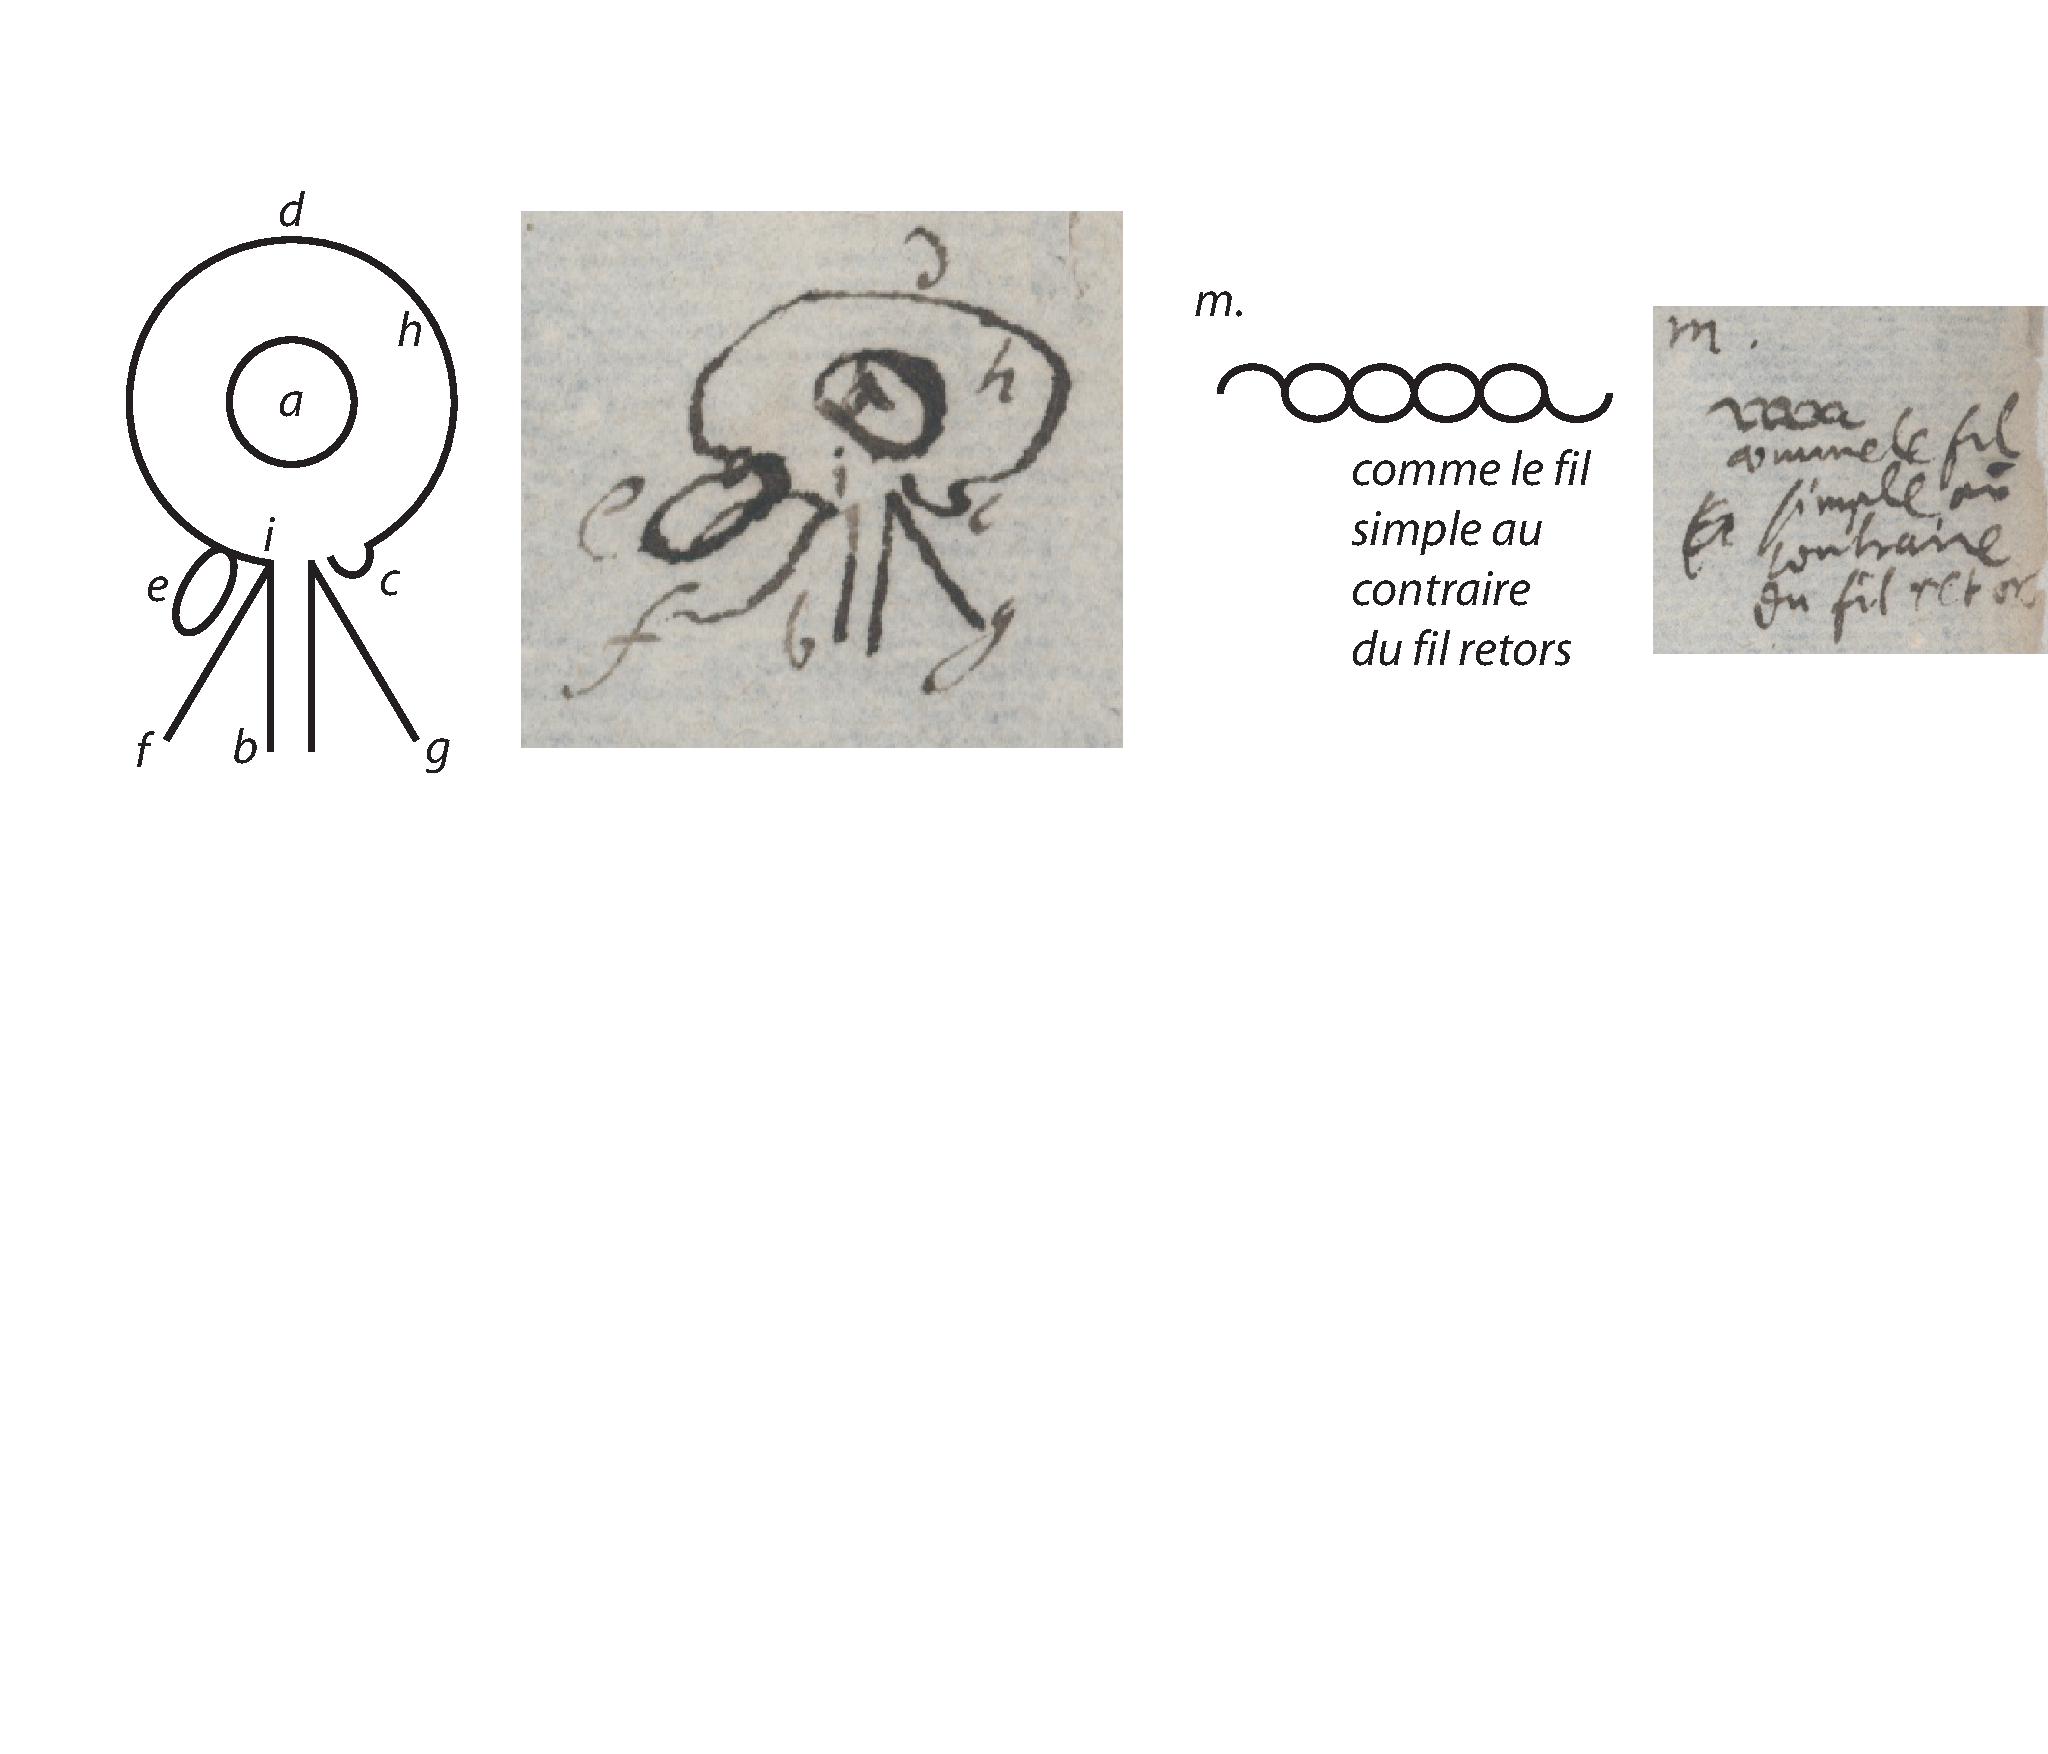
\includegraphics[width=0.5\textwidth]{images/lh0040104b_006r1.pdf}
%\caption{Bildbeschreibung}
%\end{wrapfigure}
\noindent% PR: Neuer Abschnitt.
In vitulo bimestri vel trimestri ex matrice exciso haec observavi: orificium valvulae
\edtext{erat arctissime}{\lemma{erat}\Bfootnote{\textit{(1)}\ accuratissime \textit{(2)}\ arctissime \textit{L}}}
clausum in $b.$ vasa utrinque erant in $f$ et $g$ ex cornibus $e$ et $c,$ $e$ dextrum erat longe majus altero et in id corium foetus extendebatur; non autem in sinistrum caput foetus erat versus illum, sed amnios non tam longe extendebatur sed magis in ovalem figuram in medio, ut $a$ dorsum foetus erat in $h$ umbilicus in $i$ contortus ut m ubi cutis inter cornua $c$ et $e$ erat corrugata, quoniam uterus creverat versus $d$ non autem versus $b$ et tanto arctius ejus os claudebatur;
natabat autem foetus in magna aquae copia quae cum illo includebatur, pedibusque\label{pedibusque} erat erectis, apparebatque illos nunquam adhuc fuisse incurvatos, sed crescente paulatim
\edtext{foetu fieri}{\lemma{}\Bfootnote{foetu\ \textbar\ in curvaturas \textit{gestr.}\ \textbar\ fieri \textit{L}}}
juncturas et articulos. Cartilago autem erat in genibus et aliis tam longa, quam esset ipsum os femoris vel tibiae, pedes autem erant perfecte formati, cauda etiam longior quam in adultis, item etiam penis, qui omnino usque ad umbilicum protendebatur,
\edtext{ibique erat}{\lemma{ibique}\Bfootnote{\textbar\ vero \textit{gestr.}\ \textbar\ erat \textit{L}}}
in concavum quodammodo reflexus, ut videretur ipsius nervum initio eo usque
\edtext{[perrexisse];}{\lemma{perrixisse}\Bfootnote{\textit{L \"{a}ndert Hrsg.}}}
jam autem imminui praeputiumque ibi crescere. Penis nullum habebat foramen sensibile.
Scrotum etiam erat pro mensura corporis magnum et humore tantum glutinoso plenum[,]
testes enim erant adhuc in corpore. Mammae\label{mammae} autem quatuor supra scrotum tanquam \edtext{assicularum}{\lemma{assicularum}\Cfootnote{%
Die Lesung der Handschrift ist eindeutig.
Dem Sinn nach dürfte eher \textit{acicularum} gemeint sein.
Vgl. \cite{01192}\textsc{A. Bitbol-Hespériès}, a.a.O., S.~165.}} capita, maxime conspicuae eminebant: reliquum corpus erat perfecte formatum; aures, os, nares, ut in adultis, solae oculorum palpebrae nondum erant divisae, foris tamen jam apparebant futurae rimae vestigia et tensa ibi cutis paulatim eradi videbatur: tunicae omnes foetum involventes erant pellucidae,
\edtext{[solum chorion]}{\lemma{sola corion}\Bfootnote{\textit{L \"{a}ndert Hrsg.}}} erat 
\edtext{[cotyledonibus distinctum]}{\lemma{cotelydonibus distincta}\Bfootnote{\textit{L \"{a}ndert Hrsg.}}}
per quos cotyledones apparebat foetum umbilicum ad se traxisse: mammulae enim uteri in illis erant inclusae, quae mammulae erant paulo magis albae, cotyledones paulo magis ex rubro nigricantes. Intima autem tunica quibusdam maculis instar lentis quae in aqua corrupta gignitur erat intus affecta; itemque umbilici pars exterior intra illam et foetum
\pend
\newpage
\pstart\noindent existens, erant hae maculae albae et quasi ex adipe; ut omnino viderentur esse vitium ex 
\edtext{[aqua]}{\lemma{aquae}\Bfootnote{\textit{L \"{a}ndert Hrsg.}}}
intus \edtext{[commota]}{\lemma{commotae}\Bfootnote{\textit{L \"{a}ndert Hrsg.}}} contractum.
Nulla adhuc ibi erat offa, qualis ab aliis describitur, ut inde omnino appareat offam istam esse crassius excrementum alvi quod nondum foetus egesserat, quia nimis juvenis.
\pend%
\pstart%
Apparebat etiam quam sit ridiculum fingere aquam cui foetus innatat, esse ejus sudorem; cum esset tam copiosa, et procul dubio crescente foetu diminuatur. Cornu sinistrum uteri vacuum erat, taetrum odorem exhalabat, et quasi ascarides exiguae in ejus \setline{7}initio apparebant.
[6~v\textsuperscript{o}]
\pend%
\vspace{1em}% PR: Rein provisorisch !!!
%\newpage%  PR: Rein provisorisch !!!
\pstart%
\centering%
\noindent%
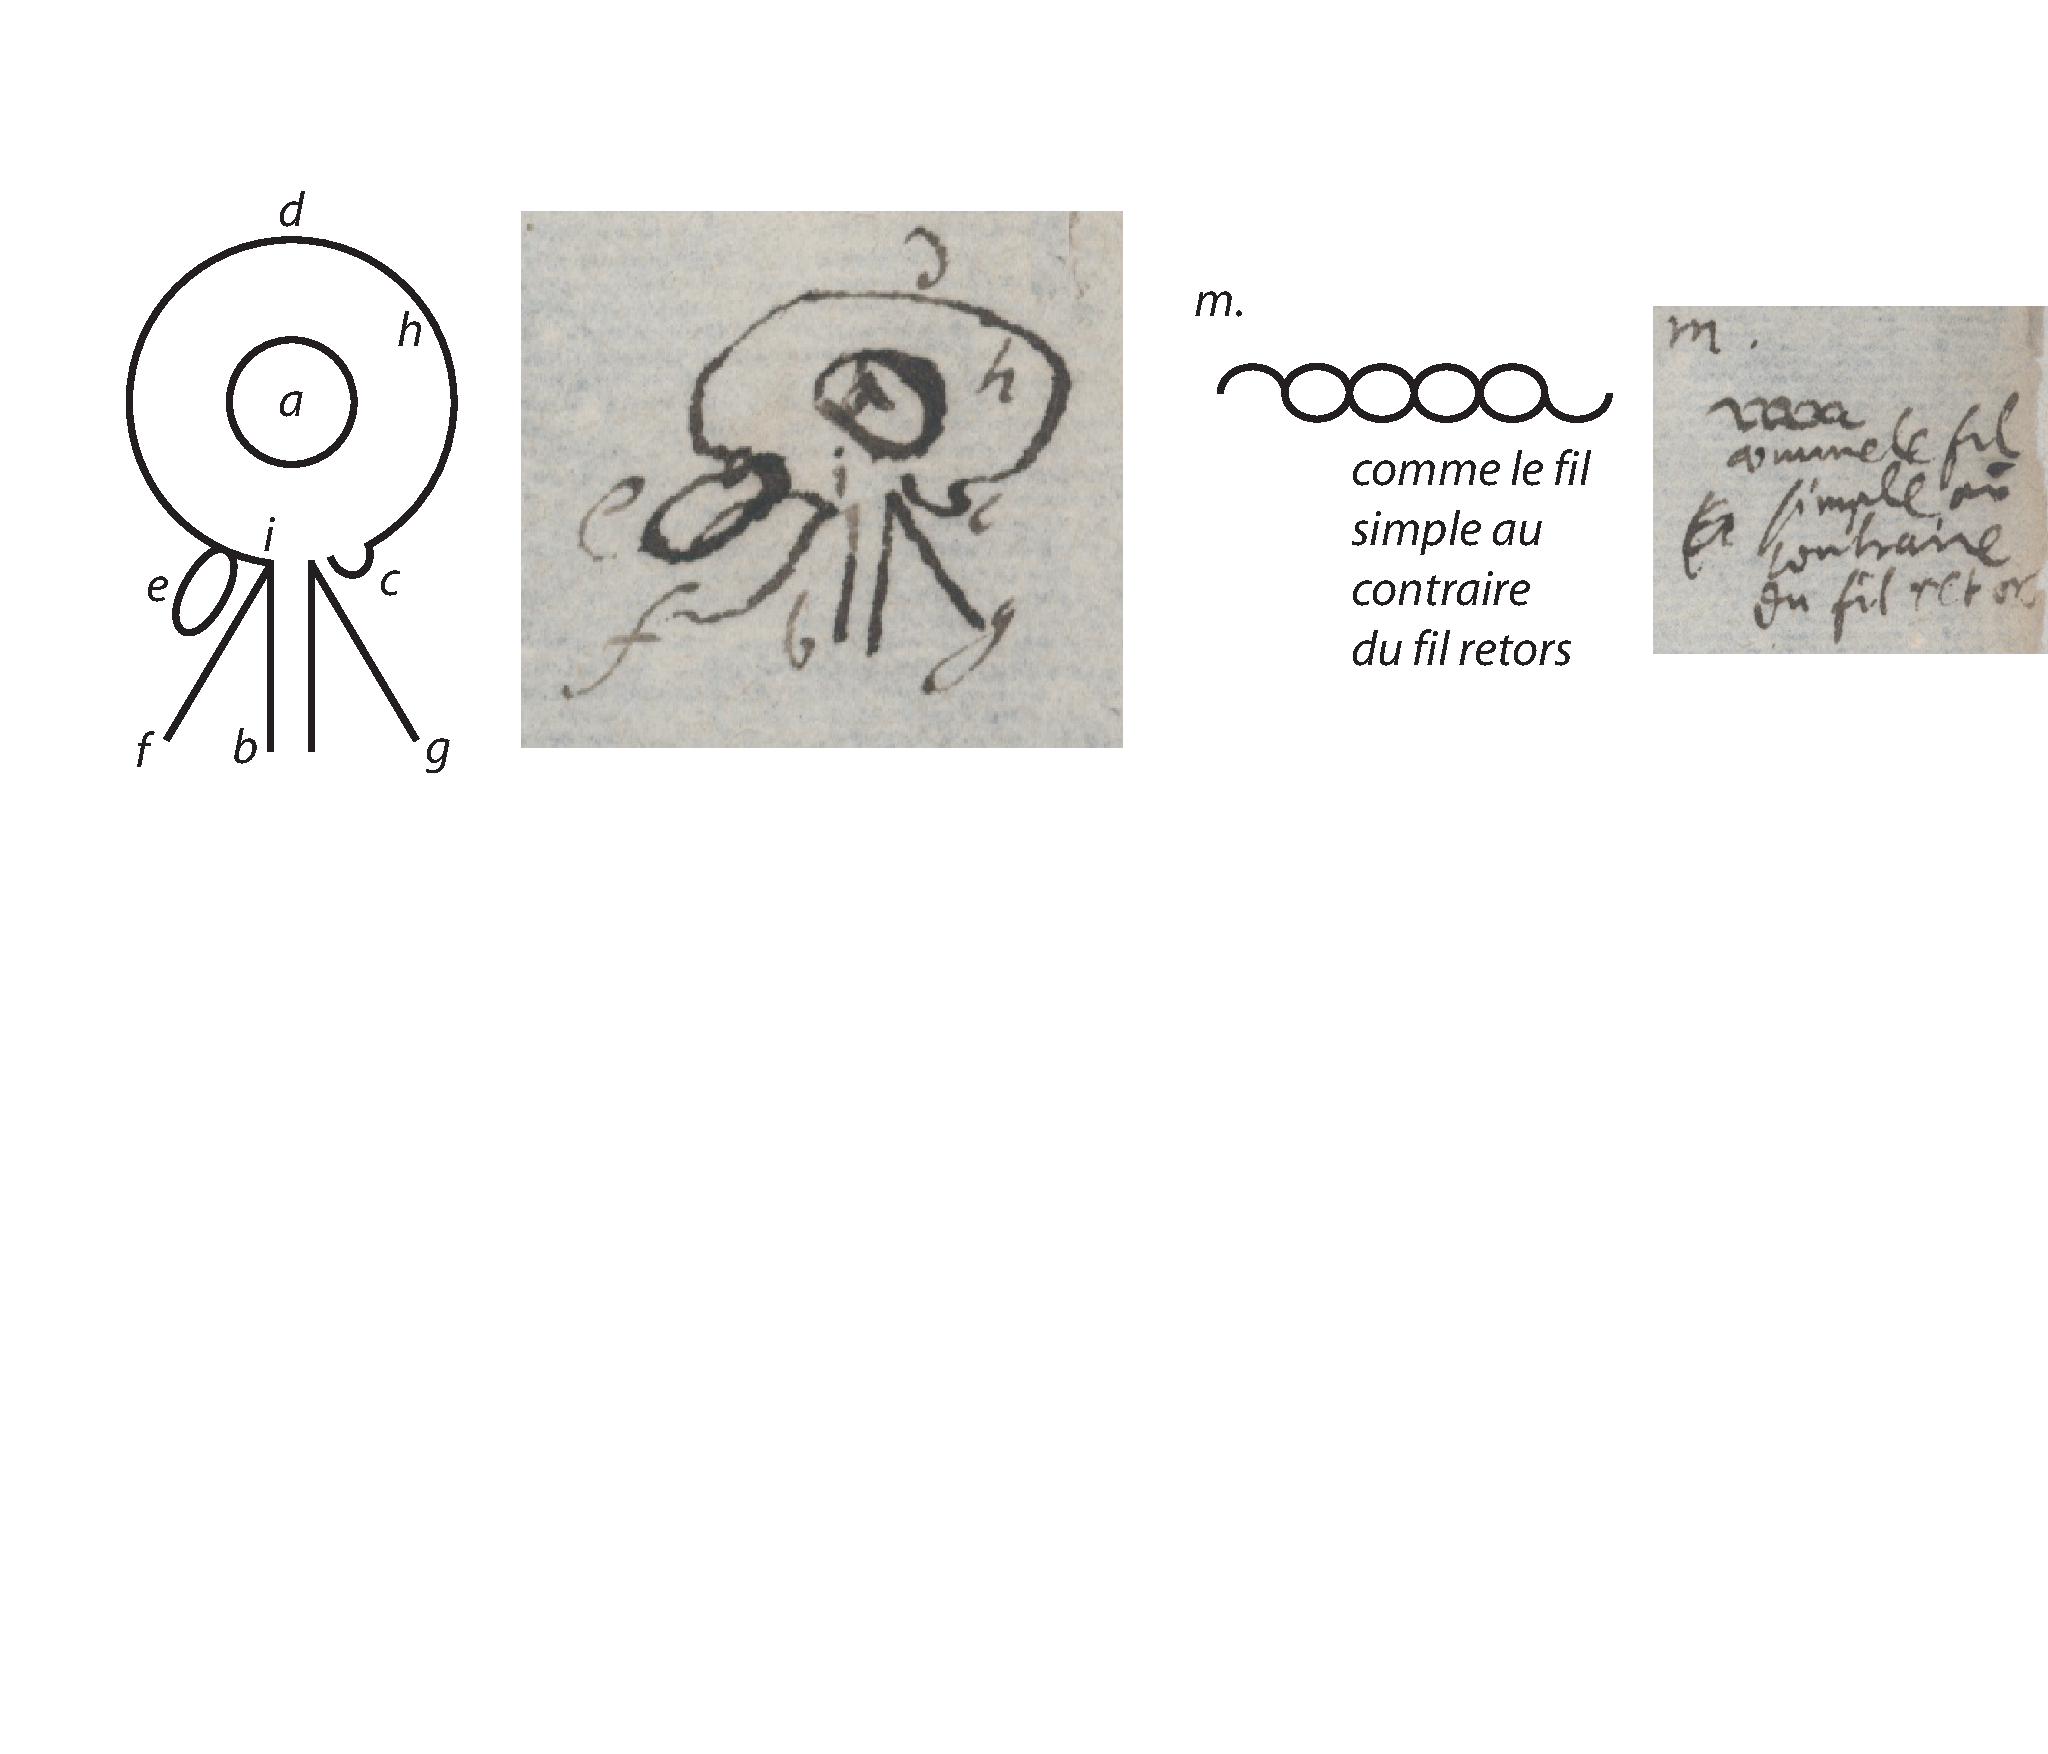
\includegraphics[trim = 0mm 2mm 0mm 0mm, clip, width=1\textwidth]{images/lh0040104b_006r1.pdf}\\
\centering [\textit{Fig. 9}]
\pend%
\vspace{1em}
%\newpage
%\vspace*{1.0em}%

%\count\Bfootins=1500
%\count\Cfootins=1500
%\count\Afootins=1500